\section{Spielübersicht}
\label{sec:ui-uebersicht}

Befindet sich der Spieler auf der Spielübersicht, so kann er sich schnell einen Überblick über das Unternehmen schaffen. Der ausgewählte Unternehmensnamen sowie das Unternehmenslogo ist im oberen Bereich des Bildschirmes zu sehen. Direkt darunter findet man eine Anzeige über die aktuelle Spielrunde und wie viele Runden noch ausstehen. 

Desweiteren hat der Spieler eine Übersicht über die verkauften Raumschiffe der letzten Runden in Form eines Säulendiagramms. Die eigenen Daten sind hierbei dem Branchendurchschnitt gegenübergestellt wodurch der Spieler die aktuelle Lage seines Unternehmens besser einschätzen kann. Rechts daneben befindet sich ein Kreis- oder Kuchendiagramm welches Aufschluss über den Marktanteil des Unternehmens gibt. Als dritte Informationsquelle auf der Spielübersicht dient der “Star der letzten Runde” sowie der “ROI der letzten Runde”. Der “Star der letzten Runde”, in dem Mockup auf \vref{img:ui-uebersicht} ist es der Millenium-Falke, kürt das meistverkaufte Raumschiffmodell der letzten Runde. Als “ROI der letzten Runde” wird der Return on Investment des Unternehmens aus den Daten der letzten Runde errechnet. Die konkrete Errechnung dieses Wertes wird in Kapitel XX genauer erläutert.

Im unteren Bereich des Bildschirmes hat der Spieler unter anderem die Möglichkeit sich über den “Spielregeln” Button noch einmal selbige durchzulesen. Sind in der aktuellen Spielrunde Ereignisse wie zum Beispiel ein Streik aufgetreten, so kann sich der Spieler diese Informationen über den Button “Informationen zur aktuellen Runde” noch einmal anschauen. Um zur ausführlichen Bewertung der letzten Spielrunde zu gelangen, klickt der Spieler auf den Button “Bewertung einsehen”. Zudem findet der Spieler auf der Spielübersicht den grün hinterlegten Button “Spielrunde einchecken” den gleichnamigen UseCase zum abschließen einer Spielrunde auslöst. 

Am linken Rand der Benutzeroberfläche befindet sich die Navigationsleiste. Über diese kann der Spieler zu den einzelnen Abteilungen wechseln und dort Informationen einsehen oder Transaktionen tätigen. Über die Navigationsleiste gelangt der Spieler beispielsweise zum Finanzwesen, welches in \ref{sec:ui-bank} beschrieben wird. 

\begin{figure}[ht]
  \centering
  \fbox{
    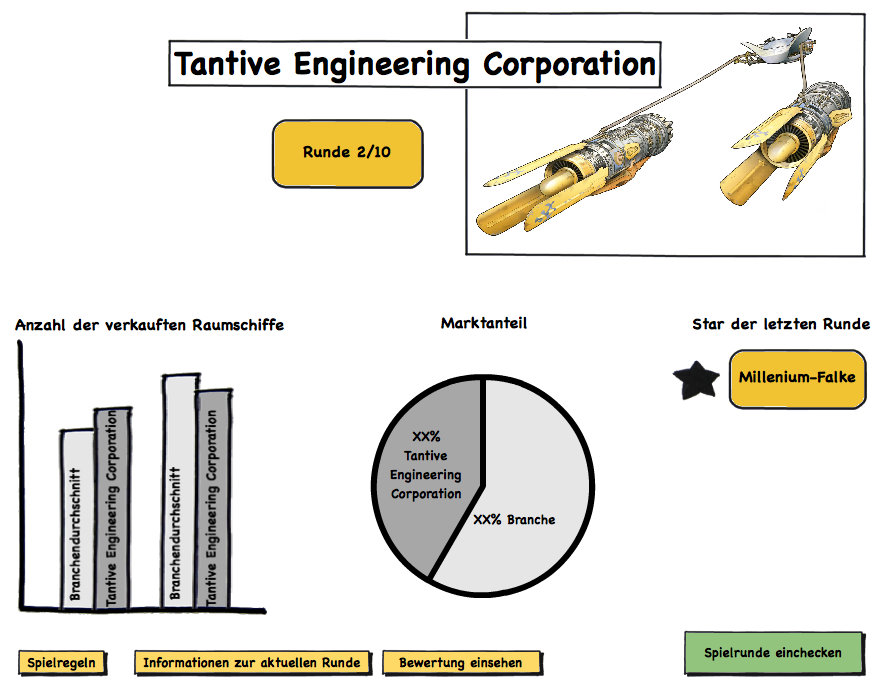
\includegraphics[width=0.9\textwidth]{40_UI/20_Uebersicht/Uebersicht.jpg}
  }
  \caption{Übersichtsbildschirm}
  \label{img:ui-uebersicht}
\end{figure}